
\section{Configuration Upgrade}

%TODO_V7 - update description

If a previous version of COMPASS has been run on the workstation, the configuration (and additional application data) might be out of date. Since the framework of COMPASS is quite sensitive on being run with the latest configuration an upgrade must be performed. \\

In older versions (before v0.6.0) this meant that the configuration was overwritten. With v0.6.0 and later, the configuration is stored in a seperate sub-folder, while configurations from older versions are deleted. \\

\includegraphics[width=0.5cm]{../../data/icons/hint.png} Please note that if the previous configuration is older than from v0.6.0, the configuration folder has to be deleted, clearing any previous changes made by the user. \\

\includegraphics[width=0.5cm]{../../data/icons/hint.png} Please note that with COMPASS version 0.5 (or later) stored configuration data sources can be exported (see \nameref{sec:config_ds_export} and imported again after the upgrade. \\

If an outdated configuration is detected, one of the following dialogs will be shown.

\begin{figure}[H]
    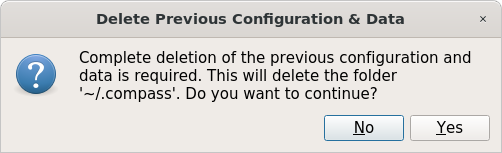
\includegraphics[width=10cm]{../screenshots/config_data_delete_update.png}
  \caption{Configuration and data delete and update}
\end{figure}

If 'Yes' is selected, the update is performed and the application starts. If 'No' is selected, the application will quit. If previous changes to an outdated configuration are of strong importance, please contact the author for support. \\

For more details about the configuration, please refer to section \nameref{sec:appendix_configuration}.
